%%%%%%%%%%%%%%%%%%%%%%%%%%%%%%%%%%%%%%%%%%%%%%%%%%%%%%%%%%%%%%%%%%%%%%%%%%%%%%%%
\chapter{Проектирование}
\label{sec:designing}
%%%%%%%%%%%%%%%%%%%%%%%%%%%%%%%%%%%%%%%%%%%%%%%%%%%%%%%%%%%%%%%%%%%%%%%%%%%%%%%%

\section{Выбор направления работы}
\label{sec:work-direction}

После изучения работы вывода типов в PyCharm было решено сосредоточиться на
проблеме вывода типов параметров функций, поскольку, несмотря на то, что PyCharm
способен определять типы параметров в некоторых случаях, например, если для них
указано значение по-умолчанию, в этой области возможностей среды разработки чаще
всего оказывается недостаточно.

Возьмем в качестве примера функцию !slugify(s)!, приведенную в
листинге~\ref{lst:slugify}:

\begin{lstlisting}[
  caption={Функция \texttt{slugify(s)}},
  label={lst:slugify}
]
def slugify(s):
    return '-'.join(s.split())
\end{lstlisting}

Посмотрев на тело функции, можно догадаться о ее назначении: разбиение строки на
слова с последующей конкатенацией их через дефис. Программист, написавший
функцию, подразумевает тип $(str) \rightarrow str$. Однако в условиях
использования в языке ``утиной'' типизации в действительности в качестве
аргумента !s! может быть использован любой объект, имеющий метод !split()!,
поэтому при отсутствии каких-либо явных аннотаций, PyCharm пессимистично считает
тип аргумента !s!  неопределенным.  Вывести тип возвращаемого значения, однако,
оказывается возможным, потому что тип возвращаемого значения стандартного метода
!join()! класса !str! известен, а то, что это метод именно класса !str! ясно из
использования литерала.  Таким образом, итоговый тип функции !slugify(s)!,
выведенный PyCharm --- $(unknown) \rightarrow str$.

Неизвестный тип параметра мог бы быть выведен из мест вызова функции, например, 
как !slugify('foo bar baz')!, но, во-первых, с целью сохранения
инкрементальности в PyCharm анализируются только вызовы функции в том же модуле,
где она объявлена, а, во-вторых, это не поможет на этапе, когда функция только
пишется, хотя в этот момент знание типа параметра !s! средой разработки
оказалось бы наиболее полезным, например, для автодополнения других методов
класса !str!, таких как, !lower()!.

\section{Основная идея алгоритма}
\label{sec:main-idea}

Главной идеей алгоритма для вывода типов параметров функций, предлагаемого в
данной работе, является использование информации об обращениях к методам и полям
параметра функции для поиска подходящих по структуре классов. 

Здесь мы придерживаемся терминологии, принятой в сообществе Python, и называем
чтение полей объекта, а также вызовы методов совместно обращениями к атрибутам
(\emph{attributes access}). В других динамически типизированных
объектно-ориентированных языках аналогичная по семантике конструкция может
называться иначе, например, \emph{передача сообщения} (\emph{message passing},
или \emph{message sending}) в Smalltalk и SELF.

С каждым параметром функции в программе можно связать \emph{структурный тип},
включающий все атрибуты параметра, к которым происходит обращение внутри
функции. Структурный тип задает необходимый интерфейс для значения параметра.
Так, для параметра !s! функции !slugify! структурный тип --- $\{split\}$, что
записывается как 

\[
    slugify.s :: \{ split \}
\]

В стандартной библиотеке Python находится несколько типов, интерфейс которых
включает метод !split!: !bytearray!, !bytes! и !str!. Каждый из
них должен быть предложен в качестве потенциального типа параметра !s!. Если
где-либо в проекте определен пользовательский класс с методом !split!, он также
должен быть включен во множество подходящих классов.

Следует отметить, что идея использования структурных типов для описания типов
объектов не является новой и уже высказывались в других работах.  Однако, только
в одной из них~\cite{Pluquet2009} по ним затем также подбирались подходящие
классы. Сложность, однако, в процессе подобного подбора классов по их
структуре представляет наследование, которое в языке Smalltalk, для которого был
разработан тот метод, проще, чем в Python, а сам алгоритм поиска классов по
иерархии наследования, предложенный авторами в работе, вступает в конфликт с
требованием инкрементальности анализа, сформулированном ранее. Мы подробнее
обсудим данную проблему в следующем разделе.

\section{Проектирование алгоритма}
\label{sec:algorithm-design}

В разделе~\ref{sec:performance-requirement} было сформулировано требование
инкрементальности анализа в среде разработки, означающее, что в процессе
изменения исходных текстов программы должны перестраиваться индексы только для
текущего редактируемого файла. Однако оказывается тяжело обеспечить сохранение этого
свойства при анализе иерархий классов, необходимом для точного вывода типов по
используемым атрибутам.

Например, авторы проекта Diamondback Ruby~\cite{Furr2009}, также введя в свой
статический анализатор объектные типы (\emph{object types}), аналогичные
используемым в данной работе структурным типам, отказались от идеи
подбора конкретных классов, аргументируя это тем, что это разрушило бы
модульность их анализа. Они пишут:

\begin{quote}
  Если бы мы хотели придерживаться только номинальных типов, мы могли бы найти
  все классы, которые имеют методы !foo! и !bar!, и затем определить в качестве
  типа параметра функции объединение всех таких классов. Однако это было чрезвычайно
  запутано и нарушило бы модульность анализа, потому что изменение множества
  классов потребовало бы обновления типа функции.

  % If we wanted to stick to nominal typing only, we could try to find all classes
  % that have methods foo and bar, and then give [an argument] a type that is the
  % union of all such classes. However, this would be both extremely messy and
  % non-modular, since changing the set of classes might require updating the type
  % of [function].
\end{quote}

Проблему неинкрементальности, или немодульности, поиска классов по атрибутам, к
которым происходит обращение нетрудно проиллюстрировать. Допустим, что в
программе на Python имеется четыре следующих определения:

\begin{lstlisting}[
  caption={Пример разрешения классов при наследовании}
]
class A:
    def foo(self):
        pass

class B(A):
    def bar(self):
        pass

class C:
    def foo(self):
        pass


def func(x):
    x.foo()
    x.bar()

\end{lstlisting}

Поясним, что в круглых скобках после имени класса при его определении
указываются его базовые классы. Например, в данном примере класс !B! наследуется
от !A!.

Так как !B! --- единственный класс в программе, в котором имеются и метод
!foo()!, и метод !bar()!, логично предположить, что он должен стать
результатом вывода типа параметра !x!  функции !func!. Однако метод !foo()!
непосредственно к классе !B!  не объявлен и доступен ему засчет
наследования от класса !A!. 

Ранее было отмечено, что быстродействие в среде
разработки достигается за счет того, что посредством индексов повторные
лексический и синтаксический разбор файлов с исходными текстами, в том числе при
поиске определений классов и функций, происходят только при необходимости. 
В идеальном случае мы хотим индекс, отображающий имя атрибута на множество
классов, которым он доступен (с учетом наследования). При наличии такого индекса
вывод типов для параметра функции будет сведен к операции пересечения таких множеств
классов для каждого из используемых атрибутов параметра.

\[
  suitableClasses_p = \bigcap_{\forall{a} \in AccessedAttributes(p)}
  ClassesWithAttribute^*(a)
\]

Представим теперь, что все четыре определения находятся в разных модулях
программы, которые индексируются независимо. Поиск атрибутов, унаследованных
классом !B! от класса !A! потребует поиска определения (разрешения имени) последнего, 
что потребует использования индексов. Мы не можем совместить
индексирование и разрешение имен, построив необходимый нам индекс. Даже если бы
это было возможно, например, через несколько проходов
индексации, изменение любого суперкласса (!A!) потребовало бы изменения
содержимого индексов для всех его наследников (!B!), что
нарушило бы свойство инкрементальности анализа.

В работе~\cite{Pluquet2009} для Smalltalk поиск классов по структурным типам осуществлялся
через обход в ширину глобальной иерархии всех классов в программе. Такой поиск
действительно может быть очень эффективным, но сам процесс построения этой
иерархии в работе не описан. Между тем, строить и постоянно удерживать в памяти,
инкрементально обновляя такую иерархию, которая в Python из-за множественного
наследования становится графом, чрезвычайно трудоемко.

Есть несколько очевидных путей решения данной проблемы. Одним из них является
использование при выводе только атрибутов, непосредственно определенных в классе
(без учета наследования). В этом случае можно было бы либо подбирать только
классы, в которых непосредственно определен по крайней мере один из используемых
атрибутов параметра, либо подбирать только те, где определены все сразу. Однако
первый вариант неизбежно привел бы к большому числу в действительности
неподходящих классов, например, класса !C! в приведенном примере, тогда как второй
исключил наследование атрибутов вовсе, и для параметра !x! не было бы
найдено ни одного подходящего класса.

Предлагаемым нами решением является построение фрагмента графа наследования при
каждом поиске классов по атрибутам параметра. Поскольку наследование атрибутов
анализируется в этом случае каждый раз заново, потребуется лишь индекс,
отображающий имя атрибута на множество классов, где он непосредственно объявлен.
Свойство инкрементальности в этом случае будет сохранено: при
изменении модуля, где определен класс, достаточно удалить его из всех множеств,
хранимых в индексе для определенных в нем атрибутов, и затем повторно внести в
индекс, когда редактирование завершено. Записей индекса для других модулей это
не затрагивает.

При наличии такого индекса первым шагом алгоритма является построение
объединения всех классов, где объявлен хотя бы один из требуемых атрибутов,
потому что все подходящие должны оказаться среди них.

\[
  candidateClasses_p = \bigcup_{\forall{a} \in AccessedAttributes(p)}
  ClassesWithAttribute(a)
\]

Корректная обработка наследования при выводе типов, между тем, также требует,
чтобы в результатах оставались лишь наиболее общие классы, т.е. находящиеся выше
всех в иерархии наследования (или в случае графа наследования крайние правые при
топологической сортировке от наследников к суперклассам). Исключение из
результатов классов-наследников при наличии подходящего по структуре базового
класса, не уменьшая точность анализа, делает результаты более удобными для
восприятия и предсказуемыми. Если этого не делать то, например, для
примера, приведенного в листинге~\ref{lst:missing-subclass}, класс !C! не будет
включен во множество классов, подходящих в качестве типа параметра !x! функции
!func!, так как в нем не объявлен непосредственно ни метод !foo()!, ни метод
!bar()!, а значит, он не содержится в индексе и не будет включен в объединение. В
результате работы нашего алгоритма единственным элементом множества будет лишь
класс !A!.

\begin{lstlisting}[
  caption={Исключение наследников из множества подходящих классов},
  label={lst:missing-subclass}
]

class A:
    def foo(self):
        pass

    def bar(self):
        pass

class B(A):
    def foo(self):
        pass
    def bar(self):
        pass

class C(A):
    pass

def func(x):
    x.foo()
    x.bar()
    
\end{lstlisting}


Псевдокод всей функции для подбора классов по структурному типу приведен на
рисунке~\ref{fig:pseudocode}.

% \begin{algorithm}
  % \caption{Алгоритм подбора классов по структурному типу.}
  % \label{lst:algorithm-pseudocode}
  % \begin{algorithmic}[1]
  % \small
  % \Function{SuggestClasses}{$accessedAttributes$}
    % \State $candidates \gets \bigcup_{\forall a \in accessedAttributes}
    % ClassesWithAttribute(a)$
    % \State $suitable \gets \emptyset$
    % \While{$candidates \ne \emptyset$}
      % \State $class \gets Pop(candidates)$
      % \State $bases \gets ResolveBases(class)$
      % \State $availableAttributes \gets Attributes(class) \cup \bigcup_{\forall{b} \in bases} Attributes(b)$
      % \If{$accessedAttributes \subseteq availableAttributes$}
        % \State $suitable \gets suitable \cup \{candidate\}$
      % \EndIf
    % \EndWhile
    % \ForAll{$class \in suitable$}
      % \ForAll{$base \in ResolveBases(class)$}
        % \If{$base \in suitable$}
          % \State $suitable = suitable \setminus \{ class \}$
          % \State \textbf{break}
        % \EndIf
      % \EndFor
    % \EndFor
  % \State \textbf{return} $suitable$
  % \EndFunction
  % \end{algorithmic}
% \end{algorithm}

\begin{figure}
\begin{center}
    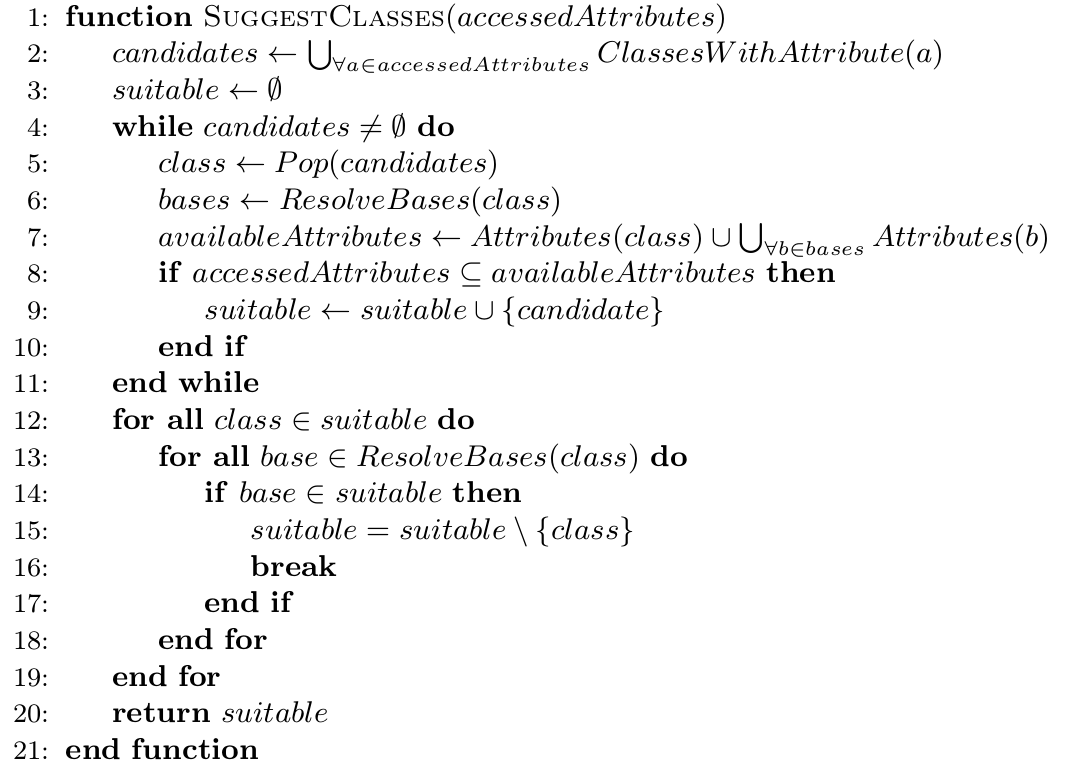
\includegraphics[width=\textwidth]{fig/pseudocode.png}
\end{center}
\caption{Псевдокод функции для подбора классов по структурному типу}
\label{fig:pseudocode}
\end{figure}

Функция $ClassesWithAttribute(attr)$ возвращает множество классов, в
которых был объявлен атрибут $attr$. При использовании индекса она
имеет сложность близкую к $O(1)$. Функция $Pop(set)$ удаляет из множества
и возвращает его произвольный элемент. Функция $Attributes(class)$ возвращает
атрибуты непосредственно объявленные в указанном классе. Предполагается, что
реализации обеих функций также имеют константную сложность. Наконец, функция
$ResolveBases(class)$ возвращает множество \emph{всех} базовых классов для
данного, и имеет сложность $O(n)$, где $n$ --- общее число известных классов.
При условии, что используется эффективная структура данных для представления
множеств, например, на основе хэш-таблиц, получение пересечения $k$ множеств
мощностью $n$ в худшем случае в строке 2 имеет сложность $O(n*k)$.  Итого,
алгоритм подбора классов по структурному типу имеет верхнюю оценку сложности
$O(n* (n + k))$, где $n$ --- количество проиндексированных классов и $k$ ---
количество атрибутов параметра, к которым происходит обращение.

Следует заметить, что можно получить значительный прирост в быстродействии, если
кэшировать результаты функции $ResolveBases(class)$ в процессе подбора классов
для одного атрибута (или до первого изменения исходных текстов программы), что
было сделано в реализации. Текст соответствующей функции Python приведен в
приложении~\ref{app:listings} листинге~\ref{lst:algorithm-python}.


В целом, поиск классов для конкретного параметра функции происходит в три этапа:

\begin{enumerate}
  \item Первоначальная индексация проекта с целью построения
    индекса, отображающего имена атрибутов на множество классов, их определяющих.
    Сохранение свойства инкрементальности анализа позволяет выполнять полную
    индексацию, включающую, например, стандартную библиотеку, только один раз,
    и впоследствии перестраивать этот индекс только для изменившихся файлов.

  \item Поиск атрибутов параметра, к которым выполняется обращение в теле
    функции. В идеальном случае такой поиск должен осуществляться
    контексто-чувствительным алгоритмом, т.е. с учетом потока управления в
    программе и псевдонимов (\emph{aliases}).

  \item Подбор классов, совместимых со структурным типом параметра.
    Выполняется при помощи описанного ранее алгоритма.

\end{enumerate}


\section{Необходимость создания прототипа}
\label{sec:prototype-necessity}

Квадратичная сложность предложенного алгоритма для подбора классов по атрибутам
ставила под сомнение применимость его в составе среды разработки, однако было
высказано предположение о том, что в действительности первоначальная фильтрация,
осуществляемая при помощи индекса классов, в которых объявлен конкретный
атрибут (функция $ClassesWithAttribute(attr)$), а также кэширование результатов
функции $ResolveBases(class)$ позволят повысить производительность до
достаточного уровня.

Для экспериментальной проверки данной гипотезы было решено разработать прототип
на Python и оценить результаты подобного вывода для нескольких реальных
проектов. Детали реализации прототипа обсуждаются в следующей главе.


% \section{Описание алгоритмов}

% \subsection{Cartesian product algorithm}
% \label{sub:CPA}

% Ole Ageseen, один из разработчиков языка SELF в 1995 предложил алгоритм
% Cartesian Product Algorithm (CPA)~\cite{Agesen1995}, позволяющий выводить
% конкретные типы аргументов для полиморфных функций. Достигается это следующим
% образом.

% Сначала собирается вся первоначально доступная информация о типах выражений и
% переменных в программе и распространяется посредством анализа графа потока
% данных (Data Flow Graph --- DFG).  Затем для каждого случая вызова функции
% информация о возможных типах аргументов используется для вывода типа ее
% возвращаемого значения. Причем поскольку из-за динамической типизации аргумент
% может принимать значение одного из нескольких возможных типов, собирается
% декартово произведение множеств возможных типов аргументов и анализ происходит
% для каждого кортежа в отдельности (отсюда название алгоритма). Каждая из
% обнаруженных комбинаций типов аргументов анализируется один раз.

% Как отмечается в работе~\cite{Madsen2007} работы O. Agessen не раскрывают
% многих аспектов практического применения алгоритма, к тому же целевой язык SELF
% имеет ряд отличий от современных высокоуровневых динамически типизированных
% языков таких как Ruby или Python. Тем не менее с момента его создания CPA
% применялся в ряде различных проектов~\cite{Madsen2007,Salib2004,Hanov},
% посвященных выводу типов в языках с динамической типизацией, и зарекомендовал
% себя как достаточно точное и эффективное решение.
